% Block 3, Question 6 (integrative, discursive): Solow saving reform x national accounts x welfare x discounting.
% Symbolic. Every closed form, sign, limit and existence claim is checked in practice-L1-L2-check-b3b.py.
% Figures: alpha = 1/3, s0 = 0.2, lambda = 1 (any admissible values; ticks carry symbolic labels only).
\questao{(15 points) Discursive. \emph{Integrative: Solow transition $\times$ national accounts $\times$ welfare
measurement $\times$ discounting.} Brazil debates a pension reform that would raise national saving for good. Take a
closed Solow economy without government: $Y=K^{\alpha}(AL)^{1-\alpha}$, $0<\alpha<1$; $A$ grows at rate $g$, $L$ at rate $n$,
capital depreciates at rate $\delta$, and $N\equiv n+g+\delta>0$. Per effective worker, $\tilde y=\tilde k^{\alpha}$ and $\hat c=(1-s)\tilde y$.
The economy is on its balanced growth path with saving rate $s_0$; at $t=0$ the reform raises the saving rate
permanently to $s_1$, with $0<s_0<s_1\le\alpha$. A representative household values the path of consumption per person,
$c(t)=A(t)\hat c(t)$, by $W=\int_0^{\infty}e^{-\rho t}\ln c(t)\,dt$, $\rho>0$. Let $D(t)\equiv\ln\hat c_1(t)-\ln\hat c_0$ be the log gap between
consumption per effective worker with the reform and without it ($\hat c_0$ is constant).}

\textbf{a)} (3 points) Using the change of variable $z\equiv\tilde k^{1-\alpha}$, find the exact path of $\tilde k$ after the reform
and its speed of convergence $\lambda$. Derive $D(t)$, its impact value $D(0)$ and its long-run value $D(\infty)$, and prove
that $D(\infty)>0$. Find the recovery time $T_R$ at which consumption regains its pre-reform level, and the condition
under which it exists.
\resolespaco
\begin{sol}
\passo{law of motion}{From $\dot K=sY-\delta K$, with $AL$ growing at $n+g$: $\dot{\tilde k}=s_1\tilde k^{\alpha}-N\tilde k$ for $t\ge0$, from the
predetermined $\tilde k(0)=\tilde k_0^*=(s_0/N)^{1/(1-\alpha)}$. With $z=\tilde k^{1-\alpha}$ this Bernoulli equation becomes linear:
\[\dot z=(1-\alpha)\tilde k^{-\alpha}\dot{\tilde k}=(1-\alpha)(s_1-Nz),\qquad z(0)=s_0/N.\]}
\passo{exact path}{Hence
\[z(t)=\frac{s_1-(s_1-s_0)e^{-\lambda t}}{N},\qquad \lambda\equiv(1-\alpha)N,\qquad \tilde k(t)=z(t)^{1/(1-\alpha)},\]
exact at any distance from the new steady state: the gap $s_1/N-z$ closes at the rate $\lambda$, which does not depend on $s$.}
\passo{consumption gap}{$\tilde y=z^{\zeta}$ with $\zeta\equiv\frac{\alpha}{1-\alpha}$, so $\hat c_1(t)=(1-s_1)z(t)^{\zeta}$ and $\hat c_0=(1-s_0)(s_0/N)^{\zeta}$. With
$b\equiv\frac{s_1-s_0}{s_1}\in(0,1)$:
\[D(t)=\ln\frac{1-s_1}{1-s_0}+\zeta\ln\Big[1+\frac{s_1-s_0}{s_0}\big(1-e^{-\lambda t}\big)\Big]=D(\infty)+\zeta\ln\big(1-b\,e^{-\lambda t}\big),\]
\[D(0)=\ln\frac{1-s_1}{1-s_0}<0,\qquad D(\infty)=D(0)+\zeta\ln\frac{s_1}{s_0},\qquad D'(t)=\frac{\alpha N\,b\,e^{-\lambda t}}{1-b\,e^{-\lambda t}}>0.\]}
\passo{long-run gain}{$D(\infty)=G(s_1)-G(s_0)$ with $G(s)\equiv\ln(1-s)+\zeta\ln s$, the log of steady-state $\hat c$ up to a constant.
$G'(s)=\frac{\alpha-s}{(1-\alpha)s(1-s)}$ is positive on $(0,\alpha)$ and zero at $\alpha$, so $G$ is strictly increasing on $(0,\alpha]$ and
$D(\infty)>0$ whenever $s_0<s_1\le\alpha$.}
\passo{recovery time}{$D$ is continuous and strictly increasing from $D(0)<0$ toward $D(\infty)$. A root exists iff $D(\infty)>0$
(intermediate value theorem; if $D(\infty)\le0$, then $D(t)<D(\infty)\le0$ at every $t$), and it is unique. Solving $D(T_R)=0$ with
$R\equiv\big(\frac{1-s_0}{1-s_1}\big)^{(1-\alpha)/\alpha}=e^{-D(0)/\zeta}$:
\[T_R=\frac1\lambda\ln\frac{s_1-s_0}{s_1-R\,s_0}=-\frac1\lambda\ln\Big[1-\frac{s_0(R-1)}{s_1-s_0}\Big],\]
well defined iff $s_1>Rs_0$, which after taking logs is $\zeta\ln(s_1/s_0)>-D(0)$, i.e.\ $D(\infty)>0$.}
\intuicao{The reform is an investment by the whole economy: consumption falls on impact by the extra share of output
saved, and the extra capital pays back gradually, at the speed $\lambda$ of the Solow transition.}
\refbib{Kurlat (2020), \S4.2 and \S4.5; Romer (2012), \S1.4 and \S1.5 (the linearized speed there is exact here for $z$).}
\rubrica{
\item Law of motion, linear equation in $z$, exact path and $\lambda$: 1 pt (linearized path used as exact: max.\ half of this line).
\item $D(t)$, $D(0)$, $D(\infty)$ and the proof that $D(\infty)>0$: 1 pt ($D(\infty)>0$ asserted without proof: 0 for that part).
\item $T_R$ with its existence condition, proved by monotonicity: 1 pt.
}
\end{sol}

\textbf{b)} (3 points) Describe the consumption and investment shares of GDP and the growth rates of GDP and of
consumption per worker along the transition. What does GDP growth say, and fail to say, about the household's
welfare? Draw $D(t)$ and $\ln\tilde y_1(t)-\ln\tilde y_0$ against $t$, marking $D(0)$, $T_R$ and the long-run values.
\resolespaco
\begin{sol}
\passo{shares}{Closed economy without government: $Y=C+I$ with $I=sY$, so $C/Y=1-s$ and $I/Y=s$ jump at $t=0$ (from $1-s_0$
and $s_0$ to $1-s_1$ and $s_1$) and then stay constant. GDP does not jump, because $\tilde k(0)$ is predetermined: the reform
changes the composition of expenditure, not its level.}
\passo{growth rates}{For $t>0$, $y=Y/L=A\tilde y$ and $c=(1-s_1)A\tilde y$ both grow at
\[\gamma(t)=g+\zeta\,\frac{\dot z}{z}=g+\frac{\alpha N(s_1-s_0)e^{-\lambda t}}{s_1-(s_1-s_0)e^{-\lambda t}},\]
which exceeds $g$, falls strictly (the numerator falls, the positive denominator rises) and tends to $g$, starting from
$g+\alpha N(s_1-s_0)/s_0$. Growth accounting attributes the excess to capital deepening: TFP growth $(1-\alpha)g$ is
unchanged and $\alpha\,\dot{\tilde k}/\tilde k=\zeta\,\dot z/z$.}
\passo{output versus consumption}{The output gap $\ln\tilde y_1(t)-\ln\tilde y_0=\zeta\ln\big[1+\frac{s_1-s_0}{s_0}(1-e^{-\lambda t})\big]$ rises from $0$ to
$\zeta\ln(s_1/s_0)$; $D(t)$ is the same curve shifted down by $-D(0)=\ln\frac{1-s_0}{1-s_1}$, the extra share of output invested.}
\passo{what GDP growth says}{GDP per worker is higher at every $t>0$ and grows faster than $g$, so GDP growth records the
benefits and none of the cost: the level fall of consumption at $t=0$ leaves GDP unchanged and shows up only in $C/Y$.
As welfare is $\int_0^\infty e^{-\rho t}D\,dt$, the same GDP path fits a gain or a loss, depending on $\rho$ (part c).}
\begin{center}
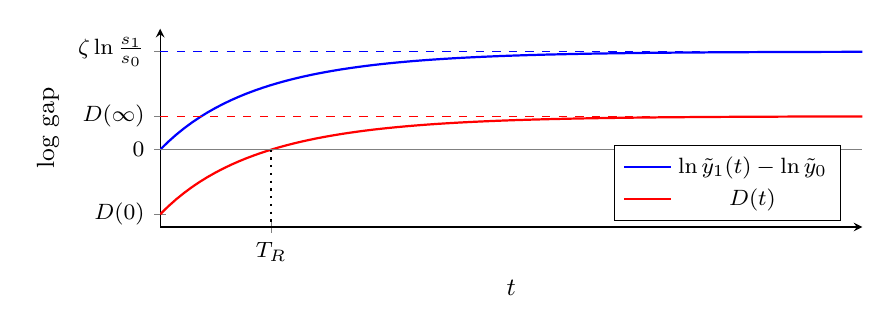
\begin{tikzpicture}
\begin{axis}[width=10.5cm,height=4.1cm,xmin=0,xmax=6,ymin=-0.16,ymax=0.25,axis lines=left,
  xlabel={$t$},ylabel={log gap},xtick={0.94738},xticklabels={$T_R$},
  ytick={-0.133531,0,0.069202,0.202733},yticklabels={$D(0)$,$0$,$D(\infty)$,$\zeta\ln\frac{s_1}{s_0}$},
  tick label style={font=\footnotesize},label style={font=\small},legend style={font=\footnotesize},legend pos=south east]
\addplot[thick,blue,domain=0:6,samples=90]{0.5*ln(1+0.5*(1-exp(-x)))};
\addplot[thick,red,domain=0:6,samples=90]{ln(7/8)+0.5*ln(1+0.5*(1-exp(-x)))};
\legend{$\ln\tilde y_1(t)-\ln\tilde y_0$,$D(t)$}
\addplot[gray,domain=0:6]{0};
\addplot[dashed,blue,domain=0:6]{0.202733};
\addplot[dashed,red,domain=0:6]{0.069202};
\addplot[dotted,thick] coordinates {(0.94738,0) (0.94738,-0.16)};
\end{axis}
\end{tikzpicture}
\end{center}
\intuicao{GDP measures what is produced, not what is consumed: saving more moves output from consumption to
investment without changing GDP, so the sacrifice shows up only in the composition of GDP.}
\refbib{Kurlat (2020), \S1.1 (expenditure approach), \S2.2 (beyond GDP) and \S5.4 (growth accounting).}
\rubrica{
\item Shares of GDP, their jump at $t=0$, GDP continuous: 0.5 pt.
\item Growth rate in closed form, proved to exceed $g$, fall and tend to $g$: 1 pt.
\item Welfare reading (benefits counted, the level cost not; the sign depends on $\rho$): 0.5 pt. No link from the national
accounts to welfare: max.\ half of the item.
\item Graph: axes, the two curves as vertical translates from $0$ and $D(0)$, with their asymptotes: 0.5 pt; $D(0)$, $T_R$ and
$D(\infty)$ marked: 0.5 pt.
}
\end{sol}

\textbf{c)} (3 points) Let $\Delta W(\rho)$ be the welfare gain of the reform and $x(\rho)$ its consumption equivalent: the permanent
proportional rise in the no-reform consumption path that the household values as much as the reform. Find $x$ in terms
of $\Delta W$, show that $x$ is strictly decreasing in $\rho$, find its limits as $\rho\to0$ and $\rho\to\infty$, and prove that there is
exactly one welfare-neutral discount rate $\rho^*$. How does $\rho^*$ depend on $N$?
\resolespaco
\begin{sol}
\passo{welfare gain and consumption equivalent}{$\ln c(t)=\ln A(0)+gt+\ln\hat c(t)$ and $\ln A(0)+gt$ is common to both paths, so
$\Delta W=\int_0^\infty e^{-\rho t}D(t)\,dt$. Scaling the no-reform path by $1+x$ adds $\int_0^\infty e^{-\rho t}\ln(1+x)\,dt=\ln(1+x)/\rho$ to $W_0$;
equating it to $\Delta W$ gives $x(\rho)=e^{V(\rho)}-1$ with $V\equiv\rho\,\Delta W$.}
\passo{integration by parts}{$D$ is bounded and $C^1$, so integrating by parts and then expanding $D'$ from (a) as a geometric
series ($0<b\,e^{-\lambda t}<1$), integrated term by term (all terms positive):
\[V(\rho)=D(0)+\int_0^\infty e^{-\rho t}D'(t)\,dt=D(0)+\alpha N\sum_{k\ge1}\frac{b^k}{\rho+k\lambda}=D(0)+\zeta\sum_{k\ge1}\frac{b^k}{\rho/\lambda+k}.\]}
\passo{monotonicity and limits}{Each term falls strictly with $\rho$, so $V$ and $x$ are strictly decreasing. As $\rho\to\infty$ each term
tends to $0$ and is bounded by $b^k/k$ (dominated convergence): $V\to D(0)$ and $x\to e^{D(0)}-1=-\frac{s_1-s_0}{1-s_0}$. As $\rho\to0$
the terms rise to $b^k/k$, and $\sum_k b^k/k=-\ln(1-b)=\ln\frac{s_1}{s_0}$ (monotone convergence): $V\to D(\infty)$ and $x\to e^{D(\infty)}-1>0$,
the steady-state gain $\hat c^*(s_1)/\hat c^*(s_0)-1$.}
\passo{welfare-neutral rate}{$V$ is continuous and strictly decreasing from $D(\infty)>0$ to $D(0)<0$. By the intermediate value
theorem there is $\rho^*$ with $x(\rho^*)=0$, unique by strict monotonicity; the reform raises welfare iff $\rho<\rho^*$.}
\passo{scaling in $N$}{$V$ depends on $\rho$ only through $\rho/\lambda$, and otherwise only on $(s_0,s_1,\alpha)$, so $\rho^*=(1-\alpha)N\varphi(s_0,s_1,\alpha)$
is proportional to $N$: $D$ depends on $t$ only through $\lambda t$, and a faster transition just changes the time unit.}
\intuicao{A patient household ($\rho\to0$) counts only the new steady state, an impatient one ($\rho\to\infty$) only the impact
loss; $\rho^*$ balances the two, in units of the transition speed $\lambda$.}
\refbib{Kurlat (2020), \S2.2 (consumption-equivalent welfare) and \S6.3 (discounting over many periods).}
\rubrica{
\item $\Delta W$ (the common trend cancels) and $x=e^{\rho\Delta W}-1$: 0.75 pt.
\item Integration by parts (or the series) and strict monotonicity, proved: 1 pt.
\item Both limits, with their reading: 0.5 pt (a limit stated without proof: 0 for it).
\item Existence and uniqueness of $\rho^*$ (intermediate value theorem plus monotonicity): 0.5 pt; $\rho^*\propto N$: 0.25 pt.
}
\end{sol}

\textbf{d)} (3 points) For a marginal reform ($s_1\downarrow s_0$), find the sign of the derivative of $\rho\,\Delta W$ with respect to $s_1$
and the discount rate $\rho_m$ at which it changes sign. Relate $\rho_m$ to the modified golden rule of a planner who
maximizes $W$, and prove that $\rho^*<\rho_m$ for every reform with $s_1>s_0$.
\resolespaco
\begin{sol}
\passo{linearized dynamics}{Write $s_1=s_0+ds$ and linearize $\dot{\tilde k}=s_1\tilde k^{\alpha}-N\tilde k$ at $\tilde k_0^*$, where $s_0\alpha(\tilde k_0^*)^{\alpha-1}=\alpha N$:
\[\frac{d\,\Delta\tilde k}{dt}=\tilde y_0^*\,ds-(1-\alpha)N\,\Delta\tilde k,\quad \Delta\tilde k(0)=0\ \Longrightarrow\ \Delta\tilde k(t)=\frac{\tilde y_0^*}{\lambda}\big(1-e^{-\lambda t}\big)\,ds,\]
which is also $\partial\tilde k(t)/\partial s_1$ of the exact path of (a) at $s_1=s_0$.}
\passo{marginal welfare}{From $\hat c=(1-s)\tilde k^{\alpha}$, $\Delta\ln\hat c=-\frac{ds}{1-s_0}+\alpha\frac{\Delta\tilde k}{\tilde k_0^*}$, and $\alpha\tilde y_0^*/\tilde k_0^*=f'(\tilde k_0^*)=\alpha N/s_0$. With
$\rho\int_0^\infty e^{-\rho t}(1-e^{-\lambda t})\,dt=\frac{\lambda}{\rho+\lambda}$:
\[\frac{\partial V}{\partial s_1}\Big|_{s_1=s_0}=-\frac{1}{1-s_0}+\frac{f'(\tilde k_0^*)}{\rho+\lambda}>0\iff\rho<(1-s_0)f'(\tilde k_0^*)-\lambda=f'(\tilde k_0^*)-N\equiv\rho_m,\]
where the last equality uses $s_0f'(\tilde k_0^*)=\alpha N$. So $\rho_m=N(\alpha-s_0)/s_0>0$, because $s_0<\alpha$.}
\passo{planner}{A planner who maximizes $W$ subject to $\dot{\tilde k}=f(\tilde k)-\hat c-N\tilde k$ cannot gain by consuming one unit less of $\hat c$ at $t$
and the proceeds $1+(f'(\tilde k)-N)\,dt$ at $t+dt$: $1/\hat c(t)=e^{-\rho\,dt}\,[1+(f'(\tilde k)-N)\,dt]/\hat c(t+dt)$, i.e.\ the Euler equation
$\dot{\hat c}/\hat c=f'(\tilde k)-N-\rho$. Its steady state is the modified golden rule $f'(\tilde k)=\rho+N$, i.e.\ $f'-\delta=\rho+n+g$. So a small
reform helps iff $\tilde k_0^*$ is below the modified-golden-rule capital of the household's own $\rho$; at $\rho_m$ it is exactly there.}
\passo{concavity in $s_1$}{With $E\equiv e^{-\lambda t}$, $D=\ln(1-s_1)+\zeta\ln\big(s_1(1-E)+s_0E\big)-\ln(1-s_0)-\zeta\ln s_0$ and
$\frac{\partial^2D}{\partial s_1^2}=-\frac{1}{(1-s_1)^2}-\frac{\zeta(1-E)^2}{(s_1(1-E)+s_0E)^2}<0$ at every $t$. So $V(s_1;\rho)=\rho\int_0^\infty e^{-\rho t}D\,dt$ is strictly concave
in $s_1$, and $V(s_0;\rho)=0$.}
\passo{$\rho^*<\rho_m$}{At $\rho_m$, $V(s_0;\rho_m)=0$ and $V_{s_1}(s_0;\rho_m)=0$, so strict concavity gives $V(s_1;\rho_m)<0=V(s_1;\rho^*)$ for every
$s_1>s_0$. Since $V$ is strictly decreasing in $\rho$ (part c), $\rho^*<\rho_m$.}
\intuicao{At the margin the reform costs $1/(1-s_0)$ now and earns $f'(\tilde k_0^*)$ on capital that builds up at rate $\lambda$, worth
$f'/(\rho+\lambda)$. Larger reforms meet diminishing returns (concavity in $s_1$), so they need more patience.}
\refbib{Kurlat (2020), \S4.3 (golden rule) and \S6.3 (Euler equation); Romer (2012), \S2.5 (modified golden rule).}
\rubrica{
\item Linearization and the marginal welfare effect in closed form: 1 pt.
\item $\rho_m=f'(\tilde k_0^*)-N$ and the modified golden rule derived from the planner's Euler equation: 1 pt (rule quoted, not
derived: max.\ a third of this line).
\item Proof of $\rho^*<\rho_m$ (concavity in $s_1$, $V_{s_1}(s_0;\rho_m)=0$, monotonicity in $\rho$): 1 pt (shown for a special case only:
max.\ half of this line).
}
\end{sol}

\textbf{e)} (3 points) \emph{Parameter analysis.} Sign, with proofs, the responses of $D(0)$, $D(\infty)$, $T_R$, $\rho^*$ and $\rho_m$ to $s_1$,
$s_0$ and $N$, and give the limits as $s_1\downarrow s_0$, at $s_1=\alpha$, and as $N\to0$ or $N\to\infty$. Compare the saving rate
that maximizes $D(\infty)$ with the one that maximizes the welfare change, and explain the difference. Draw $x(\rho)$ for two
reforms $s_1<s_1'$, marking where each crosses zero.
\resolespaco
\begin{sol}
\passo{closed forms}{$\partial D(0)/\partial s_1=-1/(1-s_1)<0$ and $\partial D(0)/\partial s_0=1/(1-s_0)>0$. $\partial D(\infty)/\partial s_1=G'(s_1)>0$ on $(s_0,\alpha)$ and $=0$ at
$\alpha$, where $D(\infty)$ peaks; $\partial D(\infty)/\partial s_0=-G'(s_0)<0$. $\rho_m=N(\alpha-s_0)/s_0$ does not depend on $s_1$ and falls with $s_0$.}
\passo{convexity in $s_0$}{$\frac{\partial D}{\partial s_0}=\frac{1}{1-s_0}-\frac{\zeta s_1(1-E)}{s_0s_1(1-E)+s_0^2E}$, whose last denominator rises with $s_0$, so $\frac{\partial D}{\partial s_0}$ rises:
$D$ is strictly convex in $s_0$ at every $t$, and so is $V$. Also $D=V=0$ when $s_1=s_0$.}
\passo{$T_R$ and $\rho^*$ in $s_1$ and $s_0$}{Fix $t=T_R$. On $[s_0,s_1]$, $D$ vanishes at both ends both as a function of the new rate
(strictly concave) and as a function of the old rate (strictly convex), so $D_{s_1}<0$ at $s_1$ and $D_{s_0}<0$ at $s_0$. With $D_t>0$,
$dT_R/ds_i=-D_{s_i}/D_t>0$ for $i=0,1$ (for $s_1$, equivalently: $\frac{R-1}{s_1-s_0}$ is the slope of a secant of the convex $R(s_1)$ from
$R(s_0)=1$, so it rises with $s_1$). The same argument on $V(\cdot\,;\rho^*)$, with $V_\rho<0$, gives $d\rho^*/ds_i=-V_{s_i}/V_\rho<0$.}
\passo{$N$}{By (a) and (c), $N$ enters only through the time scale $\lambda t$: $D(0)$ and $D(\infty)$ do not depend on $N$, $T_R\propto1/N$,
and $\rho^*$ and $\rho_m$ are proportional to $N$.}
\begin{center}
\begin{tabular}{lccc}
\toprule
 & $s_1\uparrow$ & $s_0\uparrow$ & $N\uparrow$\\
\midrule
$D(0)$ (impact loss) & $-$ & $+$ & $0$\\
$D(\infty)$ (long-run gain) & $+$ on $(s_0,\alpha)$, $0$ at $\alpha$ & $-$ & $0$\\
$T_R$ (recovery time) & $+$ & $+$ & $-$ \ ($\propto1/N$)\\
$\rho^*$ (welfare-neutral rate) & $-$ & $-$ & $+$ \ ($\propto N$)\\
$\rho_m$ (marginal threshold) & $0$ & $-$ & $+$ \ ($\propto N$)\\
\bottomrule
\end{tabular}
\end{center}
\passo{limits}{As $s_1\downarrow s_0$: $D(0),D(\infty)\to0$ but $\lambda T_R\to\ln\frac{\alpha(1-s_0)}{\alpha-s_0}>0$ (l'H\^opital on the first form of $T_R$): even a
tiny reform takes a finite time to pay back. Also $\rho^*\uparrow\rho_m$: for any $\rho<\rho_m$, $V_{s_1}(s_0;\rho)>0$, so $V(s_1;\rho)>0$, i.e.\ $\rho^*>\rho$,
for $s_1$ close to $s_0$. At $s_1=\alpha$, $D(\infty)$ and $T_R$ are largest and $\rho^*$ smallest over $(s_0,\alpha]$. As $s_0\uparrow\alpha$, $\rho_m\to0$.
As $N\to0$, $T_R\to\infty$ and $\rho^*,\rho_m\to0$; as $N\to\infty$, $T_R\to0$ and $\rho^*,\rho_m\to\infty$.}
\passo{golden rule versus welfare}{At $s_1=\alpha$, $\partial D/\partial s_1=-s_0E/\{(1-\alpha)[\alpha(1-E)+s_0E]\}<0$ at every $t$, so $V_{s_1}(\alpha;\rho)<0$ for
every $\rho>0$: a rate slightly below $\alpha$ gives more welfare. As $V$ is strictly concave in $s_1$ and $V_{s_1}(s_0;\rho)>0$ for $\rho<\rho_m$,
the best constant rate is unique and lies in $(s_0,\alpha)$; for $\rho\ge\rho_m$ it is $s_0$ (no reform). At $\alpha$, $G'(\alpha)=0$: more saving no longer raises steady-state
consumption but still lowers it at every finite date, a cost that stops counting only as $\rho\to0$, when $V\to D(\infty)$.}
\begin{center}
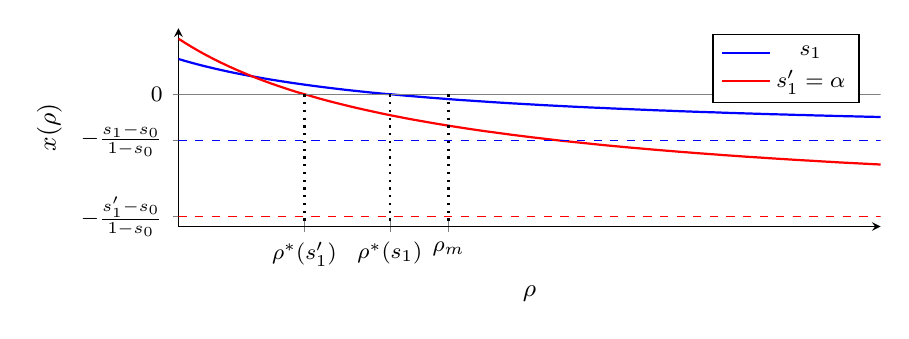
\begin{tikzpicture}
\begin{axis}[width=10.5cm,height=4.1cm,xmin=0,xmax=2.6,ymin=-0.18,ymax=0.09,axis lines=left,
  xlabel={$\rho$},ylabel={$x(\rho)$},xtick={0.466616,0.782745,1},xticklabels={$\rho^*(s_1')$,$\rho^*(s_1)$,$\rho_m$},
  ytick={-0.166667,-0.0625,0},yticklabels={$-\frac{s_1'-s_0}{1-s_0}$,$-\frac{s_1-s_0}{1-s_0}$,$0$},
  tick label style={font=\footnotesize},label style={font=\small},legend style={font=\footnotesize},legend pos=north east,
  declare function={S(\uu,\bb)=\bb/(\uu+1)+\bb^2/(\uu+2)+\bb^3/(\uu+3)+\bb^4/(\uu+4)+\bb^5/(\uu+5)+\bb^6/(\uu+6)
    +\bb^7/(\uu+7)+\bb^8/(\uu+8)+\bb^9/(\uu+9)+\bb^10/(\uu+10)+\bb^11/(\uu+11)+\bb^12/(\uu+12)+\bb^13/(\uu+13)+\bb^14/(\uu+14);}]
\addplot[thick,blue,domain=0:2.6,samples=100]{exp(ln(15/16)+0.5*S(x,0.2))-1};
\addplot[thick,red,domain=0:2.6,samples=100]{exp(ln(5/6)+0.5*S(x,0.4))-1};
\legend{$s_1$,$s_1'=\alpha$}
\addplot[gray,domain=0:2.6]{0};
\addplot[dashed,blue,domain=0:2.6]{-0.0625};
\addplot[dashed,red,domain=0:2.6]{-0.166667};
\addplot[dotted,thick] coordinates {(0.466616,0) (0.466616,-0.18)};
\addplot[dotted,thick] coordinates {(0.782745,0) (0.782745,-0.18)};
\addplot[dotted,thick] coordinates {(1,0) (1,-0.18)};
\end{axis}
\end{tikzpicture}
\end{center}
\intuicao{A more ambitious reform (higher $s_1$) or one that starts with more capital (higher $s_0$) earns a lower marginal
product, so it pays back later and needs more patience; $N$ only changes the clock. The golden-rule reform has the
largest long-run gain and the smallest $\rho^*$.}
\refbib{Kurlat (2020), \S4.3 (golden rule, dynamic efficiency); Romer (2012), \S1.4 and \S2.5.}
\rubrica{
\item Signs in $s_1$ and $s_0$, each proved (closed forms; concavity and convexity at $T_R$ and at $\rho^*$): 1.25 pt.
\item Signs in $N$ from the time scaling, and the table: 0.5 pt. Limits, including $\rho^*\to\rho_m$ and the finite $T_R$ of a
marginal reform: 0.5 pt. Golden rule versus welfare, with the proof that $V_{s_1}(\alpha;\rho)<0$: 0.25 pt.
\item Graph: two decreasing curves with the limits of (c), crossing zero in the order $\rho^*(s_1')<\rho^*(s_1)<\rho_m$: 0.5 pt.
A sign table without proofs or without the economic reading: max.\ half of the item.
}
\end{sol}
